% PUMA reconstruction — concise deck. Compile: tectonic PUMA_short.tex (figs in ./figs/)
\documentclass[aspectratio=169,12pt]{beamer}
\usetheme{Madrid}\usecolortheme{whale}
\usepackage{graphicx,booktabs}
\setbeamertemplate{navigation symbols}{}
\setbeamertemplate{footline}[frame number]
\setbeamercolor{frametitle}{bg=structure!85!black}
\setbeamerfont{frametitle}{size=\large}

\title[PUMA TPC reconstruction]{PUMA TPC --- track reconstruction}
\subtitle{Performance on the $\pi^+\pi^-$ channel}
\date{}

\begin{document}
\frame{\titlepage}

\begin{frame}{The detector}
\centering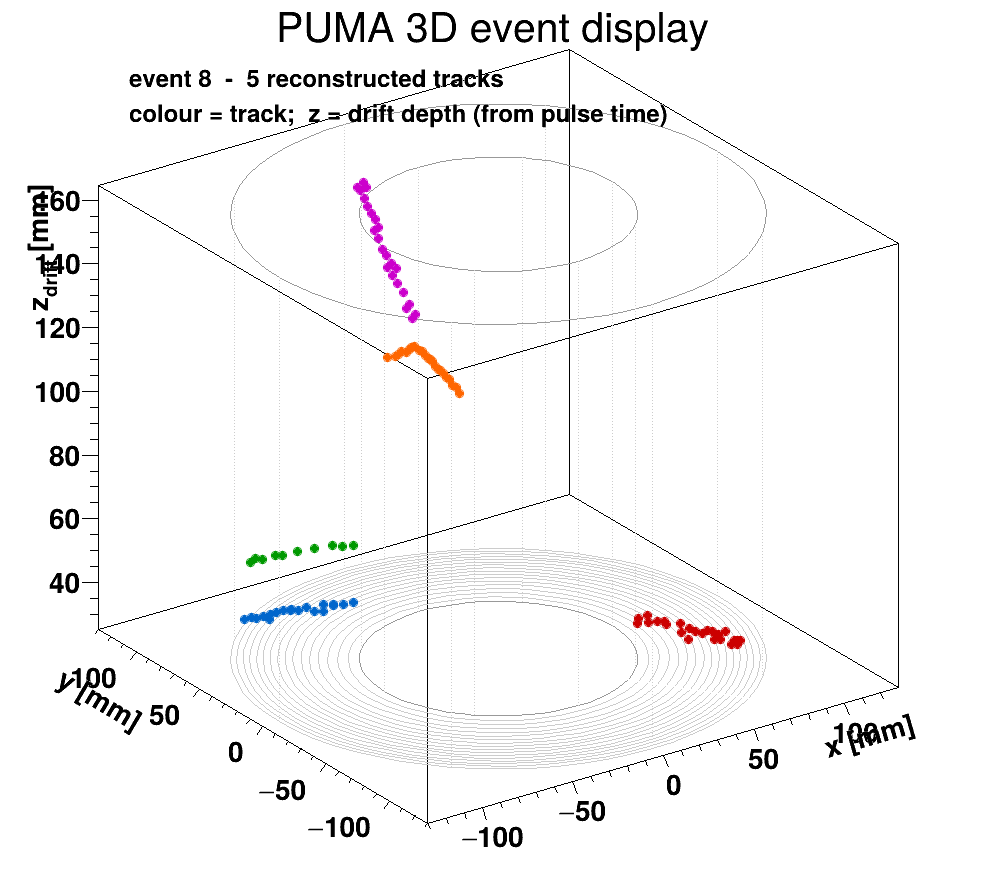
\includegraphics[height=.72\textheight]{figs/track_3d.png}\\
{\footnotesize Annular P10 TPC, 4 T. Pads $\to$ $(x,y)$; drift time $\to z$.}
\end{frame}

\begin{frame}{Reconstruction chain}
\centering
\Large pulse fit $\;\to\;$ pattern recognition $\;\to\;$ Kalman fit\\[.6em]
\normalsize
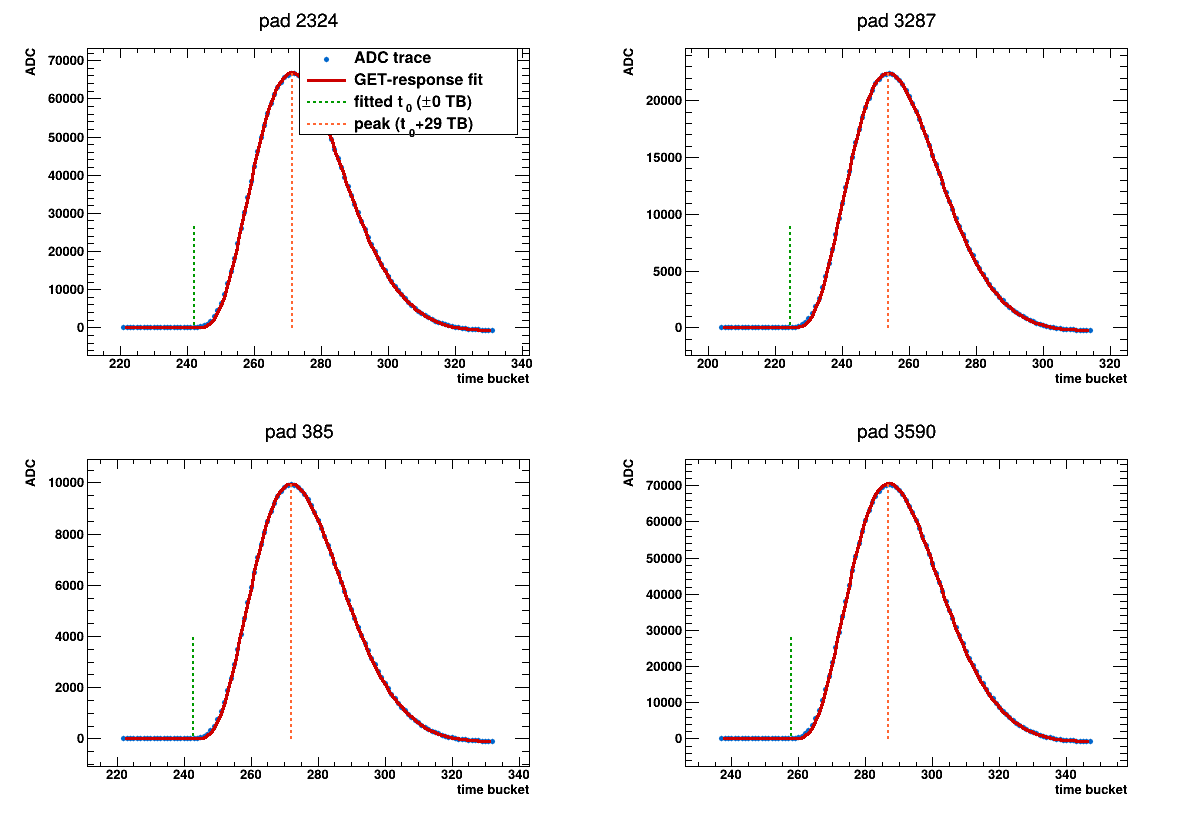
\includegraphics[height=.50\textheight]{figs/psa_fitshape.png}\\
{\footnotesize \texttt{AtPSAMultiFit} $\to$ HDBSCAN $\to$ UKF \& GENFIT.}
\end{frame}

\begin{frame}{Pattern recognition}
\centering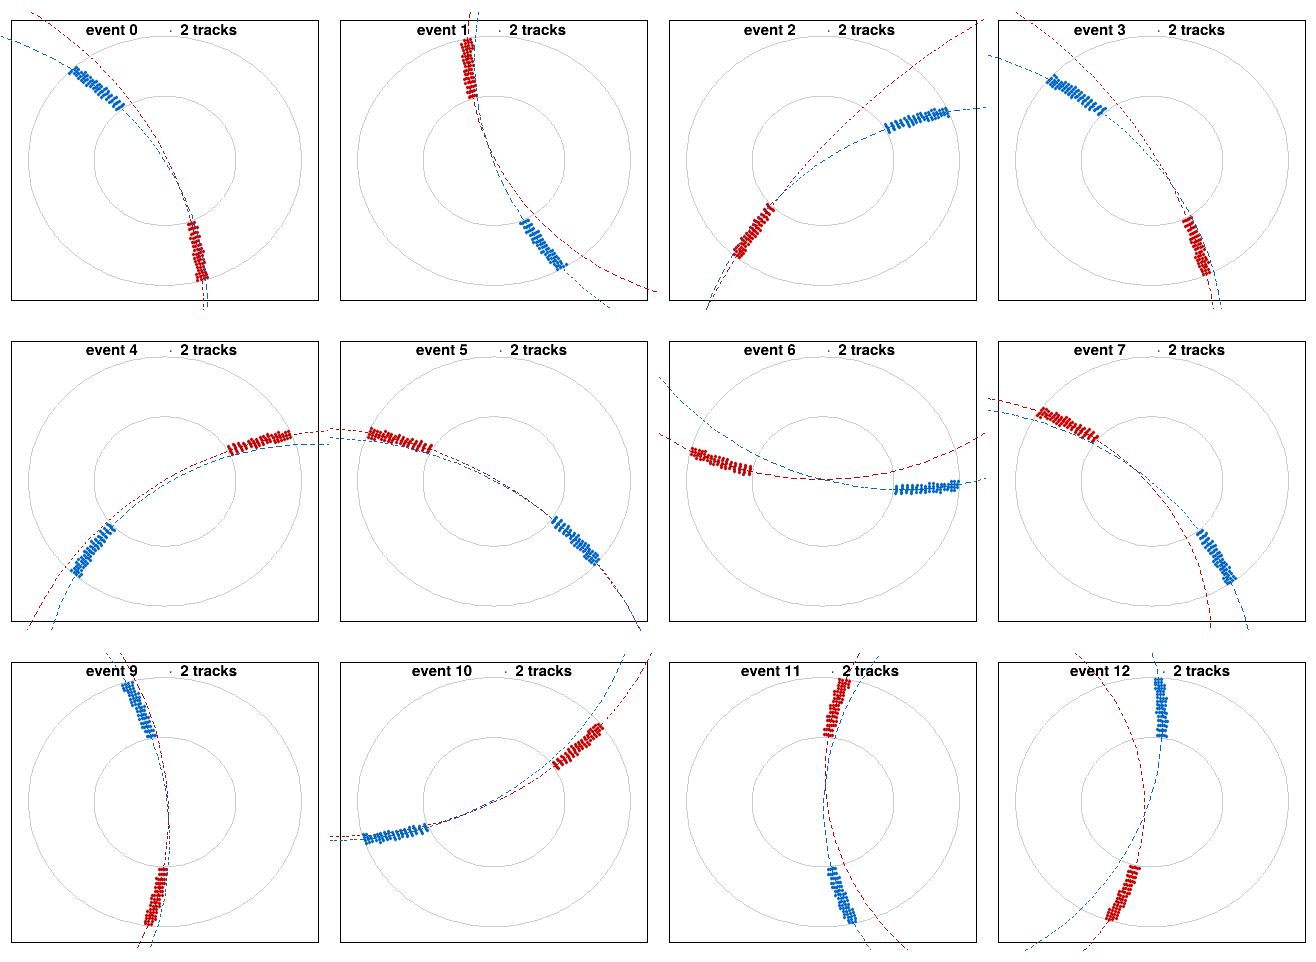
\includegraphics[height=.74\textheight]{figs/pra_examples.png}\\
{\footnotesize HDBSCAN; tracking efficiency \textbf{99.7\%}. Hits + circle fit.}
\end{frame}

\begin{frame}{Track fitting}
\centering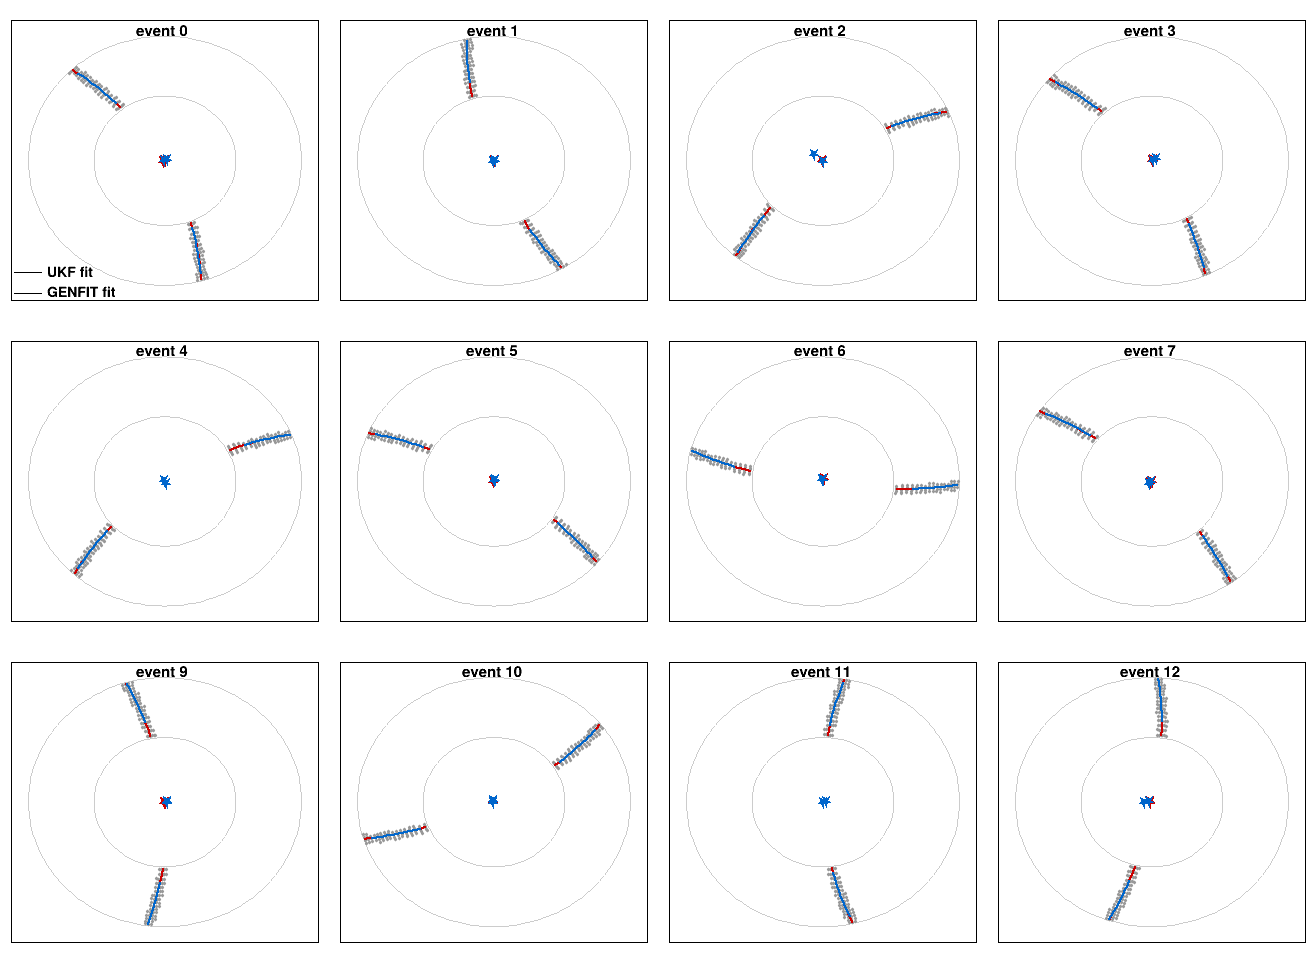
\includegraphics[height=.74\textheight]{figs/fit_examples.png}\\
{\footnotesize \textcolor{blue}{UKF} \& \textcolor{red}{GENFIT}; fitting efficiency \textbf{$\sim$100\%}.}
\end{frame}

\begin{frame}{Momentum resolution}
\centering
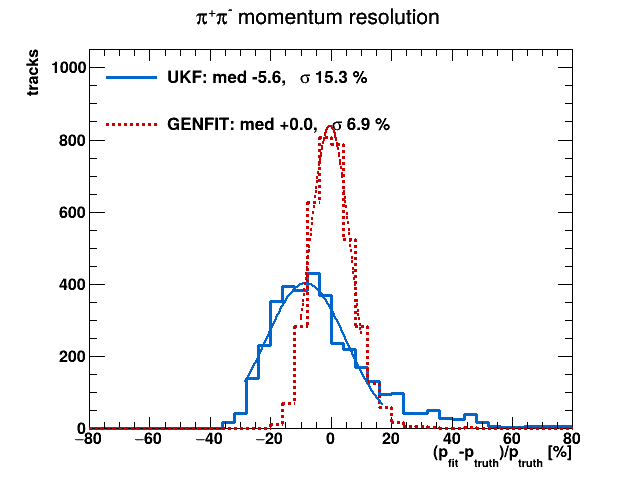
\includegraphics[height=.56\textheight]{figs/res_pi_dlc_dp.png}\\[.3em]
\begin{tabular}{lcccc}\toprule
 & momentum $\sigma$ & $\theta$ $\sigma$ & vertex $\sigma_z$ & charge\\\midrule
UKF    & 15\% & 2.0$^\circ$ & 0.50 mm & 99.5\%\\
GENFIT & \textbf{7\%} & 1.8$^\circ$ & 0.47 mm & 99.6\%\\\bottomrule
\end{tabular}
\end{frame}

\begin{frame}{Resolution vs momentum}
\centering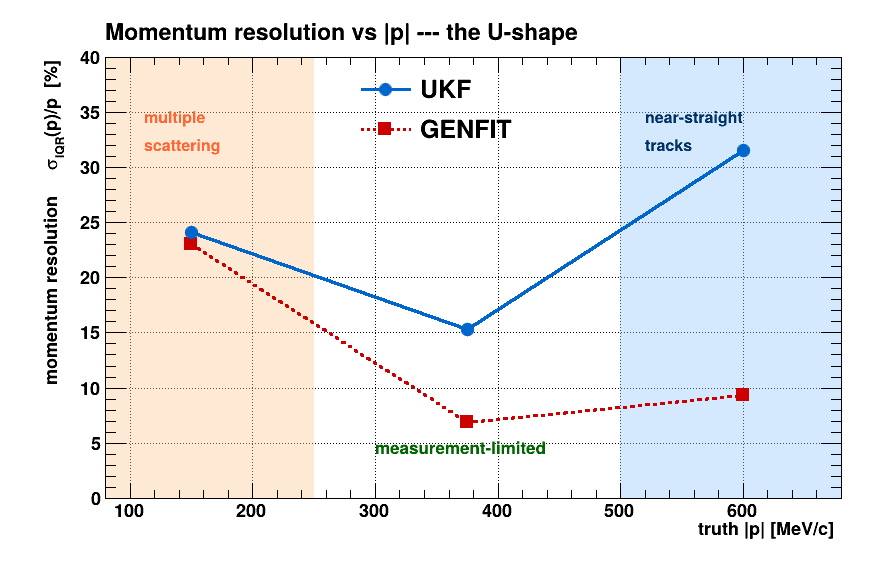
\includegraphics[height=.60\textheight]{figs/res_vs_p.png}\\
{\footnotesize \textbf{U-shape}, best at 375--500 MeV/c. Low $p$: \textbf{multiple scattering} ($\propto 1/p\beta$) --- an irreducible floor (both fitters converge). High $p$: \textbf{near-straight} tracks, little curvature to measure.}
\end{frame}

\begin{frame}{Particle ID: $\pi^+/\pi^-$}
\centering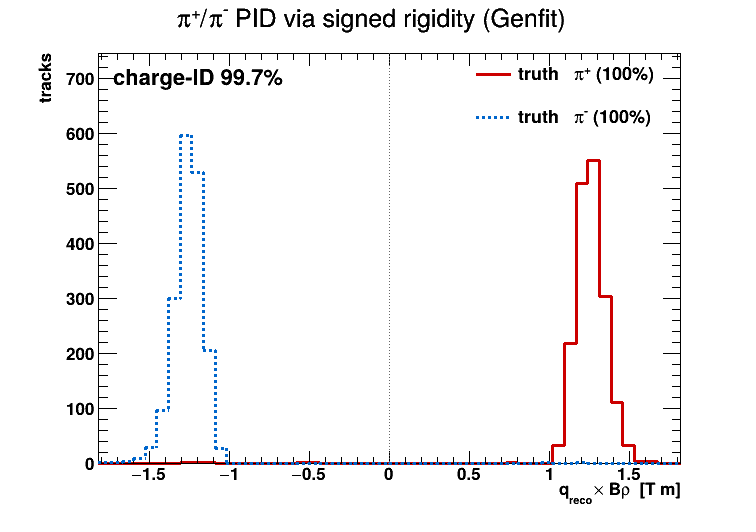
\includegraphics[height=.66\textheight]{figs/pid_pipm_dlc.png}\\
{\footnotesize Charge sign from rigidity: \textbf{99.7\%}, $14.5\,\sigma$ separation.}
\end{frame}

\begin{frame}{Summary}
\centering
\begin{tabular}{lc}\toprule
tracking efficiency & 99.7\%\\
fitting efficiency & $\sim$100\%\\
momentum resolution (GENFIT) & \textbf{7\%}\\
polar-angle resolution & 1.8$^\circ$\\
vertex resolution $\sigma_z$ & 0.5 mm\\
charge / $\pi^+\pi^-$ ID & 99.7\%\\\bottomrule
\end{tabular}\\[.8em]
{\footnotesize Full chain runs natively; GENFIT is the stronger fitter.}
\end{frame}

\end{document}
